%% Springer Nature LaTeX template (sn-jnl.cls, December 2024 package).
%% Target: Discover Artificial Intelligence.
%%
%% Build:  pdflatex sn-article && bibtex sn-article && pdflatex sn-article && pdflatex sn-article
%% or:     make -f Makefile.springer
%%
%% Numbers below are transcribed from artefacts/*.json. Before submitting run
%%     python scripts/check_paper_numbers.py --strict
%% which re-derives them and fails on drift.

%% Discover AI requires numbered citations in square brackets, e.g. [1-3, 7].
%% The 'Numbered' option selects that reference style in sn-jnl.cls.
\documentclass[pdflatex,sn-basic,Numbered]{sn-jnl}

%% sn-jnl.cls does not load these itself, and this manuscript uses
%% \bigcup / \bigl / \varepsilon (amsmath) and includes figures (graphicx).
\usepackage{amsmath}
\usepackage{amssymb}
\usepackage{graphicx}
\usepackage{multirow}
% The class loads neither; algorithm/algpseudocode are needed for the
% pseudocode in Section 4 and do not clash with sn-jnl.cls (which defines no
% `algorithm' float of its own).
\usepackage{algorithm}
\usepackage{algpseudocode}

%% Architecture diagram (Fig. 1) is drawn in TikZ rather than embedded as a
%% raster: it keeps lettering vector-sharp at any zoom, matches the body font
%% automatically, and lets the data-flow constraints be drawn explicitly.
\usepackage{tikz}
\usetikzlibrary{arrows.meta,positioning,fit,backgrounds,calc,shapes.geometric}

%% Set \tikzfigurefalse to fall back to the pre-rendered raster (figures/Fig1.png)
%% if the submission system's TeX installation misbehaves with TikZ.
\newif\iftikzfigure
\tikzfiguretrue

%% Monochrome palette. The diagram is printed black-only, so the distinction
%% between pipeline stages is carried by FILL LEVEL and LINE STYLE rather than
%% by hue. This is the convention in the game-theoretic XAI literature, it
%% survives greyscale printing and photocopying, and it is colourblind-safe by
%% construction -- a point the reviewer raised about the other figures.
%% Fill levels are kept >=4 percentage points apart so they remain separable
%% after halftoning.
\definecolor{snSource}{gray}{0.00}
\definecolor{snCand}{gray}{0.00}
\definecolor{snGame}{gray}{0.00}
\definecolor{snShap}{gray}{0.00}
\definecolor{snFuse}{gray}{0.00}
\definecolor{snGrey}{gray}{0.00}

%% Springer requires figure lettering at 8-12pt. Note that sn-jnl.cls
%% redefines the size macros: \tiny is 5pt and \footnotesize is 7pt, both of
%% which would VIOLATE that rule. We therefore set explicit point sizes here
%% rather than relying on the relative macros.
\newcommand{\snFigMain}{\fontsize{9}{10.5}\selectfont}
\newcommand{\snFigSub}{\fontsize{8}{9.5}\selectfont}

\tikzset{
  %% snbox takes a grey fill level as its argument: stages that produce the
  %% paper's output (the game, the Shapley values) are drawn heavier than the
  %% stages that merely prepare data, so the eye lands on them first.
  snbox/.style={
    rounded corners=2pt, draw=black, line width=0.7pt, fill=black!#1,
    inner sep=4pt, align=center, font=\snFigMain, text width=32mm},
  %% The estimand the paper is about: same geometry, heavier rule.
  snboxmain/.style={
    rounded corners=2pt, draw=black, line width=1.3pt, fill=black!#1,
    inner sep=4pt, align=center, font=\snFigMain, text width=32mm},
  %% Data folds: square corners, so fold vs pipeline stage is a SHAPE
  %% distinction and not only a shading one.
  snfold/.style={
    sharp corners, draw=black, line width=0.5pt, fill=white,
    inner sep=3pt, align=center, font=\snFigSub, text width=26mm},
  snflow/.style={-{Stealth[length=4.5pt,width=3.5pt]}, draw=black,
    line width=0.8pt},
  sndata/.style={-{Stealth[length=4.5pt,width=3.5pt]}, draw=black,
    line width=0.5pt, dashed, dash pattern=on 2.2pt off 1.6pt},
  snlbl/.style={font=\snFigSub, inner sep=1.6pt, text=black},
}
\graphicspath{{figures/}}

\theoremstyle{thmstyleone}
\newtheorem{theorem}{Theorem}
\newtheorem{proposition}[theorem]{Proposition}
\newtheorem{lemma}[theorem]{Lemma}

\theoremstyle{thmstyletwo}
\newtheorem{property}{Property}
\newtheorem{remark}{Remark}

\raggedbottom

\newcommand{\G}{\mathcal{G}}
\newcommand{\Cu}{C_u}
\newcommand{\NDCG}{\mathrm{NDCG@10}}
\newcommand{\LOO}{\mathrm{LOO}}

\begin{document}

\title[Exact Ranking-Stage Source Attribution]{SignalShap: Exact
Ranking-Stage Attribution of Sources in Hybrid Recommenders}

\author*[1]{\fnm{Mouad} \sur{Louhichi}}\email{mouad\_louhichi@um5.ac.ma}
\author[1]{\fnm{Redwane} \sur{Nesmaoui}}\email{redwane.nesmaoui@um5.ac.ma}
\author[1]{\fnm{Mohamed} \sur{Lazaar}}\email{mohamed.lazaar@ensias.um5.ac.ma}

\affil*[1]{\orgdiv{National Higher School of Computer Science and Systems
Analysis (ENSIAS)}, \orgname{Mohammed V University in Rabat},
\city{Rabat}, \country{Morocco}}

\abstract{Source ablation and Shapley attribution are often treated as
competing estimates of the same quantity: how much a component of a hybrid
recommender is worth. We show that they answer different questions, and that
conflating them leads to the wrong instrument for the decision at hand.

We present \emph{SignalShap}, which recasts source attribution as a five-player
cooperative game --- collaborative filtering, content, popularity, recency, and
sequential order --- whose payoff is a fixed-candidate normalised discounted
cumulative gain at rank~10 on a coalition-independent candidate set. With five
players the Shapley value follows from exact enumeration of all $2^5=32$
coalitions, so the aggregation carries no sampling error. We validate the
implementation against constraints known in advance: six analytic games with
closed-form Shapley vectors reproduce exactly, duplicate injection recovers
symmetry to numerical precision, and efficiency holds to
$6.9\times10^{-18}$.

Across three timestamped corpora spanning a $36\times$ density range, every
system contains at least one source on which the two rules disagree in
\emph{sign}, and which source diverges is corpus-specific. But in an end-to-end
retirement simulation, leave-one-out predicts the true cost of removing a
source \emph{better} than Shapley ($\tau=1.00$ against $0.20$ and $0.60$).
SignalShap allocates the value of a declared ranking-stage game; leave-one-out
estimates the effect of removal from the deployed system. We therefore claim
credit allocation, not retirement guidance, and identify candidate recall as a
necessary applicability test that only one of our three corpora passes. Code
and every backing artefact are released.}

\keywords{Shapley value, cooperative game theory, recommender systems,
explainable AI, credit assignment, hybrid recommendation}

\maketitle

\section{Introduction}\label{sec:intro}

A production hybrid recommender is an ensemble of architecturally distinct
scorers. A collaborative-filtering component exploits co-occurrence, a content
component exploits item metadata, a popularity component exploits global
frequency, a recency component exploits temporal locality, and a sequential
component exploits order. Engineering decisions --- which component to invest in, which to retire --- rest
on estimates of how much each contributes. We show in
Section~\ref{sec:estimands} that these are two distinct questions requiring
different instruments, and that this paper addresses the first. In
practice those estimates come from \emph{leave-one-out} (LOO) \emph{ablation}:
disable one component, measure the drop in ranking quality, and attribute that
drop to the component.

Ablation answers a narrower question than the one being asked. It measures what
is lost when a component is removed from the \emph{complete} system, which is
the right quantity only when components contribute independently. Real hybrids
do not: popularity and implicit-feedback collaborative filtering overlap by
construction, since matrix factorisation on implicit signals is strongly
popularity-driven. When two components carry overlapping information, removing
either alone changes little, and both appear worthless. What practitioners
actually want is each component's contribution averaged over the situations in
which it might be needed --- including those where no substitute is available.

Cooperative game theory answers exactly that question. The Shapley
value~\citep{shapley1953} is the unique credit assignment satisfying
efficiency, symmetry, null-player, and additivity, and it evaluates each player
against \emph{every} coalition rather than only against the grand coalition.
Its adoption in machine learning has been broad~\citep{lundberg2017,
covert2021explaining}, but almost entirely at the granularity of \emph{input
features}. Our object of study is different: the players are
\emph{architectural sources}, and the payoff is a ranking metric.

Figure~\ref{fig:workflow} summarises the pipeline. That change of granularity
buys something unusual. Feature-level Shapley must
approximate --- the coalition lattice over hundreds of features is intractable,
so KernelSHAP and its relatives sample and inherit estimator variance. With
five architectural sources the lattice has $2^5 = 32$ elements and the exact
closed form is a short sum, which we compute directly. Second, and more
importantly, \emph{verifiability}: a small player set makes it possible to
construct cases in which the attribution must satisfy a known constraint, and
check that the method does. Section~\ref{sec:recovery} does this for symmetry
and efficiency on real fitted games.

\subsection{Contributions}

\begin{itemize}
\item \textbf{C1.} A precisely declared ranking-stage cooperative game over
      heterogeneous recommender sources, with a coalition-independent candidate
      set that makes $v(S)$ comparable across coalitions, a per-user
      formulation, and exact enumeration for small source sets
      (Section~\ref{sec:game}).
\item \textbf{C2.} A formal characterisation of source allocation under
      redundancy: efficiency and per-user decomposition, a counterexample
      showing the redundancy--positivity property is \textbf{false} without
      monotonicity, a corrected two-sided $\varepsilon$-substitutability
      result, and the observation that Shapley credit is \emph{not} conserved
      under replication (Section~\ref{sec:theory}).
\item \textbf{C3.} A validation protocol for source attribution combining
      analytic games with known Shapley vectors, controlled duplicate
      injection, and efficiency, null-player, and additivity diagnostics
      (Sections~\ref{sec:recovery} and~\ref{sec:validating}). These establish
      that the aggregation is implemented correctly --- a precondition for
      interpreting anything computed with it, and one the field rarely checks.
\item \textbf{C4 (primary).} An empirical comparison of three estimands ---
      refitted-head ranking-stage, fixed-head, and end-to-end retrieval ---
      showing that Shapley allocation and leave-one-out removal cost answer
      \emph{different questions}. On both corpora where an end-to-end ground
      truth can be measured, leave-one-out predicts retirement cost better than
      Shapley ($\tau = 1.00$ against $0.20$ and $0.60$). We pair this with
      candidate recall as a necessary applicability test, and report where our
      own method should not be used (Sections~\ref{sec:results}
      and~\ref{sec:estimands}).
\end{itemize}

\paragraph{What this paper does not claim}
We do not claim that attribution-derived fusion weights improve ranking
quality: they are practically equivalent to a globally tuned head under a
pre-specified margin, and we report that negative result in
Appendix~\ref{app:fusion} rather than as a contribution. We make no
state-of-the-art claim against LightGCN or SASRec; those models appear as
contextual references only, and received smaller tuning budgets than a
performance comparison would require. And we do not claim that the sign of an
attribution prescribes retaining or removing a source --- Section~\ref{sec:estimands}
shows it does not.

\begin{figure}[t]
\centering
\iftikzfigure
%% resizebox is a no-op while the picture fits; it guarantees the figure can
%% never exceed the text block if node sizes are later changed.
\resizebox{\linewidth}{!}{%
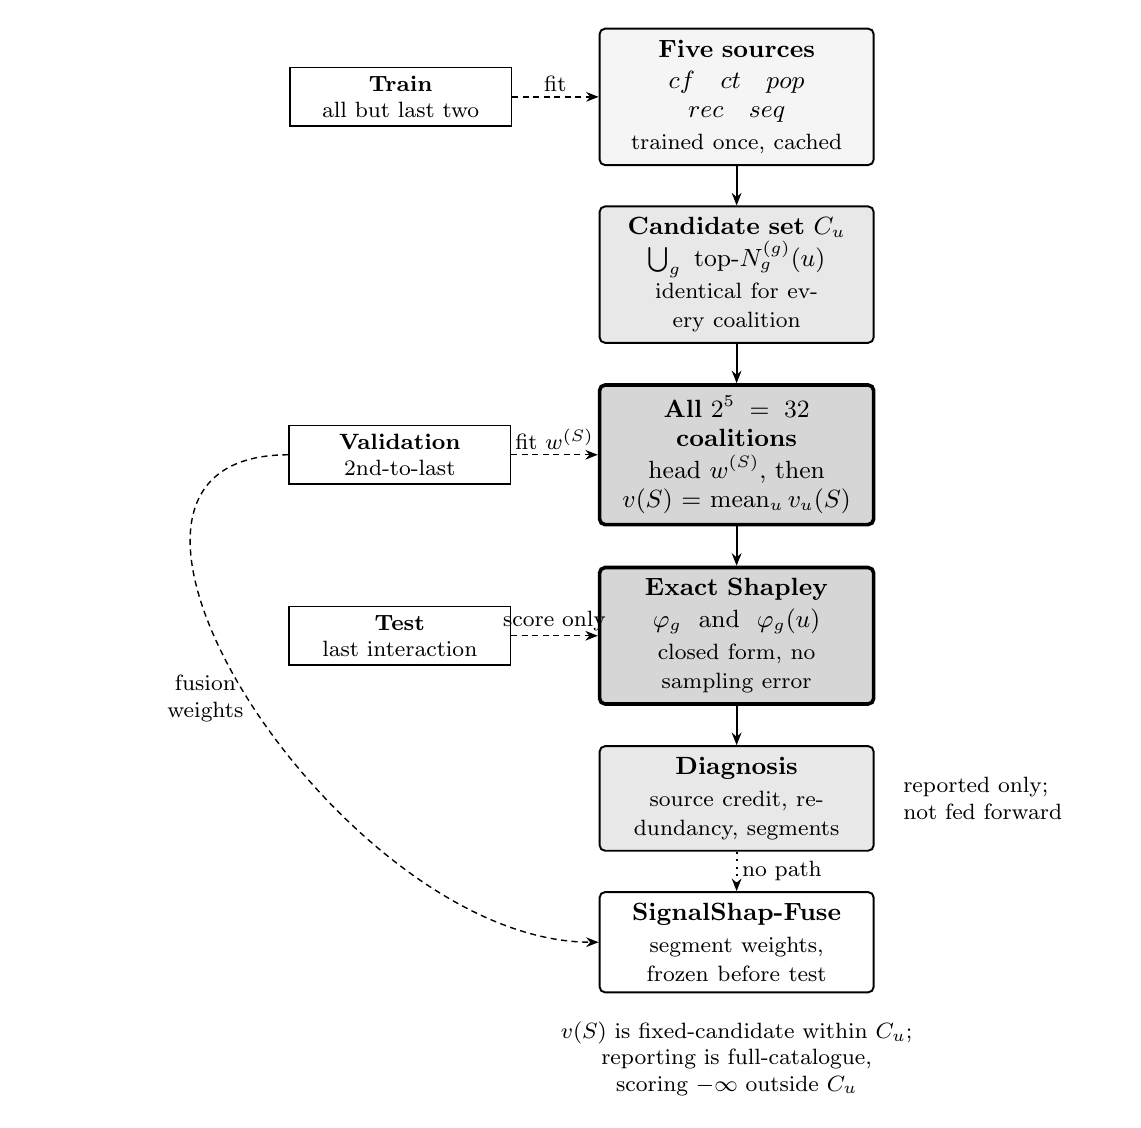
\begin{tikzpicture}[node distance=5mm]

%% ------------------------------------------------------------------
%% Vertical layout: the pipeline reads top-to-bottom in the main
%% column, with the three data folds as a narrow rail on the left.
%% Kept inside \linewidth so it cannot overflow the text block.
%% ------------------------------------------------------------------

%% --- pipeline spine (centre) --------------------------------------
\node[snbox=4] (src)
  {\textbf{Five sources}\\[1pt]
   $cf$\quad $ct$\quad $pop$\quad $rec$\quad $seq$\\[1pt]
   {\snFigSub trained once, cached}};

\node[snbox=9, below=of src] (cand)
  {\textbf{Candidate set} $\Cu$\\[1pt]
   $\bigcup_g\ \text{top-}N_g^{(g)}(u)$\\[1pt]
   {\snFigSub identical for every coalition}};

\node[snboxmain=16, below=of cand] (game)
  {\textbf{All $2^5=32$ coalitions}\\[1pt]
   head $w^{(S)}$, then
   $v(S)=\mathrm{mean}_u\, v_u(S)$};

\node[snboxmain=16, below=of game] (shap)
  {\textbf{Exact Shapley}\\[1pt]
   $\varphi_g$ \ and \ $\varphi_g(u)$\\[1pt]
   {\snFigSub closed form, no sampling error}};

\node[snbox=9, below=of shap] (diag)
  {\textbf{Diagnosis}\\[1pt]
   {\snFigSub source credit, redundancy, segments}};

\node[snbox=0, below=of diag] (fuse)
  {\textbf{SignalShap-Fuse}\\[1pt]
   {\snFigSub segment weights, frozen before test}};

\draw[snflow] (src)  -- (cand);
\draw[snflow] (cand) -- (game);
\draw[snflow] (game) -- (shap);
\draw[snflow] (shap) -- (diag);

%% --- data folds (left rail) ---------------------------------------
\node[snfold, left=11mm of src]  (train) {\textbf{Train}\\{\snFigSub all but last two}};
\node[snfold, left=11mm of game] (val)   {\textbf{Validation}\\{\snFigSub 2nd-to-last}};
\node[snfold, left=11mm of shap] (test)  {\textbf{Test}\\{\snFigSub last interaction}};

\draw[sndata] (train) -- node[snlbl,above]{fit} (src);
\draw[sndata] (val)   -- node[snlbl,above]{fit $w^{(S)}$} (game);
\draw[sndata] (test)  -- node[snlbl,above]{score only} (shap);

%% validation also supplies the fusion weights -- never the Shapley output
\draw[sndata] (val.west) to[out=180,in=180,looseness=1.15]
  node[snlbl,left,pos=0.5,align=center]{fusion\\weights} (fuse.west);

%% --- the separation that prevents circularity ---------------------
%% Dotted, and the ONLY dotted edge in the figure, so the negative claim it
%% encodes -- that Shapley output never reaches the fusion weights -- reads
%% without colour.
\draw[{Stealth[length=4.5pt,width=3.5pt]}-, draw=black, line width=0.7pt,
      dotted] (fuse.north) -- node[snlbl,right]{no path} (diag.south);

\node[snlbl, right=3mm of diag.east, anchor=west, align=left, text width=26mm]
  {reported only;\\not fed forward};

%% --- protocol note ------------------------------------------------
\node[snlbl, below=3mm of fuse.south, align=center, text width=64mm]
  {$v(S)$ is fixed-candidate within $\Cu$;\\
   reporting is full-catalogue, scoring $-\infty$ outside $\Cu$};

\end{tikzpicture}%
}
\else

\includegraphics[width=\linewidth]{Fig1.png}
\fi
\caption{The SignalShap pipeline, with data folds made explicit. Sources are
fitted on train; every coalition head $w^{(S)}$ and every fusion weight is
fitted on \emph{validation}; test interactions are used only to score. The
candidate set $\Cu$ is the union of all sources' top-$N$ lists and is identical
for every coalition, so differences in $v(S)$ reflect fusion within $S$ rather
than retrieval from a pool that favours it. Because $v(S)$ is evaluated on test
interactions, the Shapley output is reported as diagnosis and is deliberately
\emph{not} an input to the fusion weights (dotted arrow); that separation is
what keeps the downstream comparison of Appendix~\ref{app:fusion}
non-circular}\label{fig:workflow}
\end{figure}

\subsection{Research questions}

\begin{description}
\item[RQ1] Does a fixed-candidate, coalition-independent cooperative game over
  architectural sources admit an exact additive decomposition of ranking
  quality, and does the implementation satisfy the Shapley axioms on real
  fitted games?
\item[RQ2] Does source-level Shapley attribution differ materially from
  leave-one-out ablation, and is the difference associated with measured
  redundancy between sources?
\item[RQ3] Do the ranking-stage, fixed-head, and end-to-end estimands agree,
  and which of them predicts the measured cost of retiring a source?
\end{description}

\paragraph{What is not in this paper} Graph-neural or Transformer players;
causal attribution; online or counterfactual evaluation. All attribution is
\emph{within} the declared game and the fixed candidate set.

\section{Related Work}\label{sec:related}

\paragraph{Shapley values in machine learning}
SHAP~\citep{lundberg2017} unified additive feature attribution; extensions
cover trees~\citep{lundberg2020}, data valuation~\citep{ghorbani2019}, and
federated contribution~\citep{wang2020federated}.
Surveys~\citep{covert2021explaining, rozemberczki2022shapley} note that
essentially all practical estimators sample, because the coalition lattice is
exponential in the number of players. Our setting sidesteps this: five players,
32 coalitions, closed form.

\paragraph{Feature-level XAI versus source-level attribution}
SHAP, LIME~\citep{ribeiro2016}, and Integrated
Gradients~\citep{sundararajan2017} answer ``which input features moved this
prediction?''. We answer ``which architectural component earned the system's
ranking quality?''. The unit of attribution differs, the payoff is a ranking
metric rather than a scalar output, and the actionable decision differs --- ours
is a build-or-retire decision about a subsystem.

\paragraph{Attribution to model components and to performance}
Closer to our unit of analysis than feature-level XAI is work attributing
behaviour to \emph{model components} rather than inputs. Neuron
Shapley~\citep{ghorbani2020neuron} treats individual neurons as players with a
performance payoff, and ensemble games~\citep{rozemberczki2021ensemble} treat
whole classifiers as players and allocate ensemble accuracy among them --- the
closest structural precedent for what we do, since both take trained models as
players and a performance metric as the characteristic function. Related work
attributes changes in \emph{performance} rather than individual
predictions~\citep{zhang2023performance,shah2024coar}. Our framing of Shapley
as ``almost entirely feature-level'' would be wrong; the correct statement is
that component-level valuation exists and that this paper extends it to
architectural sources in a ranking system.

\paragraph{Shapley for ranking}
A recent line develops Shapley attribution specifically for ranked outputs.
RankSHAP~\citep{chowdhury2025rankshap} axiomatises feature attribution for
learning-to-rank and evaluates against ranking metrics;
RankingSHAP~\citep{heuss2025rankingshap} gives a listwise formulation;
ShaRP~\citep{pliatsika2025sharp} defines games for score, rank, top-$k$, and
pairwise-preference outcomes. Within recommendation, triplet
importance~\citep{he2024triplet} values training triplets by ranking utility.
All of these take \emph{features} or \emph{training data} as players and
approximate the value by sampling. SignalShap differs on both axes: the players
are architectural source models, and with five players the value is computed by
exhaustive enumeration rather than estimated. The distinguishing design choice
is the coalition-independent candidate set with a coalition-refitted fusion
head, which makes coalition values comparable across a subset lattice in a
two-stage retrieval-then-rank architecture --- a construction these works do not
require because their players do not affect retrieval.

\paragraph{Which Shapley, and which game}
Shapley uniqueness holds \emph{once a game is fixed}; it does not select the
game. Sundararajan and Najmi~\citep{sundararajan2020many} show that plausible
operationalisations differ materially, which is why we state our candidate
construction, coalition head, and baseline explicitly and treat them as
declared modelling choices rather than as the canonical formulation.
Alternative cooperative values --- Banzhaf and other
semivalues~\citep{karczmarz2022banzhaf} --- and interaction-aware extensions
such as the Shapley interaction index~\citep{grabisch1999interaction} and the
Shapley--Taylor index~\citep{sundararajan2020shapleytaylor} are natural
comparators. Because redundancy between sources is central to our setting we
evaluate Banzhaf, a uniform semivalue, and the Grabisch--Roubens interaction
index rather than deferring them (Section~\ref{sec:alternatives}); we do not
compute Shapley--Taylor, and Section~\ref{sec:alternatives} explains why the
distinction matters.
Replication sensitivity of Shapley allocations~\citep{han2022replication} is
directly relevant to our duplicate-injection design and is discussed in
Section~\ref{sec:recovery}.

\paragraph{Hybrid recommenders and ablation practice}
Burke's taxonomy~\citep{burke2002hybrid} classifies hybridisation strategies;
weighted and feature-combination hybrids dominate practice. Evaluation of
component worth is near-universally by
ablation~\citep{zangerle2022evaluating}. Recent recommender XAI
work~\citep{zhang2020explainable} explains \emph{recommendations}, not
\emph{architectures}.

\section{The Cooperative Game}\label{sec:game}

Let $\G = \{cf, ct, pop, rec, seq\}$ with $|\G| = 5$.

\subsection{Coalition-independent candidates}

For user $u$ and source $g$, let $\text{top-}N_g^{(g)}(u)$ be that source's own
top-$N_g$ items, and set
\begin{equation}
\Cu \;=\; \operatorname{Trunc}_{N_{\max}^{(d)}}\!\Bigl(
\bigcup_{g \in \G} \operatorname{top-}\!N_g^{(g)}(u) \Bigr),
\qquad |\Cu| \le N_{\max}^{(d)} .
\label{eq:cand}
\end{equation}
Here $d$ indexes the dataset, since the cap is pre-registered per corpus
(Table~\ref{tab:preconditions}), and $\operatorname{Trunc}_{N}$ retains the
first $N$ items after sorting the union by the key
$(\text{best rank of the item across } g\in\G,\ \text{source order in }\G,\
\text{item index})$. All three components are seed-independent, so $\Cu$ is
deterministic; the bound in~\eqref{eq:cand} holds by construction rather than
by assumption. Sources contribute equal depth, $N_g = N$ for all $g$, with $N$
grown until the union reaches the cap.

This choice is load-bearing. The obvious alternative --- draw one candidate pool
from the full fused scorer --- is \emph{invalid}, because it hands the grand
coalition a retrieval pool selected in its own favour. Every $v(S)$ for
$S \subsetneq \G$ is then evaluated on items chosen to suit $\G$, so $v(\G)$ is
inflated relative to all of them. Since Shapley values are built entirely from
differences $v(S \cup \{g\}) - v(S)$, that inflation contaminates every
attribution. Under the union design each coalition scores an identical item
set, so differences in $v(S)$ reflect \emph{fusion within $S$}, not retrieval.
We retain the rejected design as an ablation and quantify the bias it induces.

\paragraph{Candidate recall is a ceiling, not a detail}
A test item outside $\Cu$ contributes zero to $\NDCG$ by construction.
Candidate recall $\Pr[\text{test}_u \in \Cu]$ therefore upper-bounds every
ranking metric downstream, and we report it before any attribution number
(Table~\ref{tab:preconditions}).

\subsection{Characteristic function}

Let $z_{u,g,i}$ be the per-user, per-source $z$-normalised score. For coalition
$S$, $\hat{s}_{u,i}(S) = \sum_{g \in S} w_g^{(S)} z_{u,g,i}$ with $w^{(S)}$ a
head fitted on the validation fold, and
Let $y_{u,i} = \mathbb{1}[i = i_u^{\mathrm{test}}]$ for $i \in \Cu$ be the
binary relevance vector, let $\pi_u(S)$ be the ranking of $\Cu$ induced by
$\hat{s}_{u,\cdot}(S)$ under a deterministic tie rule (descending score, then
ascending item index), and let $\pi_u^{0}$ be a frozen permutation of $\Cu$
drawn once. Define the \emph{per-user} baseline and game
\begin{equation}
b_u = \NDCG(\pi_u^{0}; y_u), \qquad
v_u(S) = \NDCG(\pi_u(S); y_u) - b_u, \qquad
v(S) = \frac{1}{|\mathcal{U}|}\sum_{u} v_u(S).
\label{eq:game}
\end{equation}
If $i_u^{\mathrm{test}} \notin \Cu$ then $y_u = \mathbf{0}$ and
$\NDCG(\cdot\,; y_u) = 0$ for every ranking, so $v_u(S) = -b_u = 0$; such users
contribute zero to every coalition and are the reason candidate recall bounds
all downstream metrics. Because $v_u(\varnothing) = \NDCG(\pi_u^{0}; y_u) - b_u
= 0$ \emph{for every user}, the empty coalition is zero per user and not merely
on average, which is what Property~\ref{prop:decomp} requires.

The coalition head is the ridge solution on the validation fold,
\begin{equation}
w^{(S)} \;=\; \arg\min_{w \in \mathbb{R}^{|S|}}
\sum_{u} \frac{1}{|\Cu|}\bigl\| \mathbf{y}^{\mathrm{val}}_u - Z_u^{(S)} w \bigr\|_2^2
\;+\; \lambda \|w\|_2^2 ,
\label{eq:head}
\end{equation}
where $Z_u^{(S)} \in \mathbb{R}^{|\Cu| \times |S|}$ stacks the $z$-normalised
scores of the sources in $S$ over $i \in \Cu$, and
$\mathbf{y}^{\mathrm{val}}_u \in \{0,1\}^{|\Cu|}$ marks the user's held-out
validation interaction. The $1/|\Cu|$ factor matters: candidate sets differ in
size across users, and without it users with larger pools would dominate the
fit. Weights are unconstrained and no intercept is fitted. Test interactions
are never used to fit $w^{(S)}$.

The frozen permutation $\pi_u^{0}$ is drawn once under a fixed seed and reused
for every coalition, user, and experiment; the empty-coalition ranking is
defined to be that same permutation.

\paragraph{The baseline is a modelling choice, not a normalisation}
An earlier version of this manuscript asserted that $\varphi_g$ is invariant to
$b_u$ because it cancels in every marginal difference. That is false, and we
correct it here. The baseline cancels in $v_u(S\cup\{g\}) - v_u(S)$ only when
$S \neq \varnothing$. For $S = \varnothing$ the marginal is
$v(\{g\}) - 0 = \operatorname{mean}_u[\NDCG(\pi_u(\{g\}); y_u) - b_u]$, which
retains it. Because the empty set carries Shapley weight $w(0) = 1/n$, changing
the baseline shifts \emph{every} $\varphi_g$ by exactly $-\Delta/n$, where
$\Delta$ is the change in the mean baseline.

We verified this rather than reasoning about it: re-running the identical game
with a different permutation seed changed the mean baseline by $-0.000796$ and
shifted all five MovieLens values by $+0.00015926 = 0.000796/5$, agreeing to
eight decimal places, and moved $\varphi_{ct}$ across zero. The same mechanism
explains the constant offset between the attribution values reported in
Section~\ref{sec:results} and those recomputed inside the retirement
experiment of Section~\ref{sec:estimands}, whose games draw separate
baselines.

Three consequences. First, $b_u$ is a declared component of the game and must
be reported with it, which we now do. Second, efficiency is unaffected:
$\sum_g \varphi_g = v(\G)$ holds because $v(\G)$ shifts by the same amount.
Third, and most importantly for how this paper should be read, source
\emph{rankings} and the sign-disagreement analysis of
Section~\ref{sec:results} are unchanged by a uniform shift only where the
values are well separated; $\varphi_{ct}$ on MovieLens sits within $10^{-4}$ of
zero and its sign is therefore not a stable finding. We rely on it nowhere.

\paragraph{The regularisation strength is frozen}
$\lambda$ is chosen once on a pilot and never tuned per coalition.
Per-coalition tuning is not benign: it is optimistic bias that \emph{grows with
$|S|$}, since larger coalitions have more parameters and more opportunity to
overfit the held-out interaction. That would inflate $v(\G)$ relative to small
coalitions --- the same pathology as a grand-coalition candidate pool, arriving
by a different route.

\subsection{Exact aggregation}

\begin{equation}
\varphi_g \;=\; \sum_{S \subseteq \G \setminus \{g\}}
\frac{|S|!\,(|\G| - |S| - 1)!}{|\G|!}
\bigl[ v(S \cup \{g\}) - v(S) \bigr],
\end{equation}
a closed-form sum over $2^5 = 32$ coalitions; for $n=5$ the weights by $|S|$
are $(\tfrac15, \tfrac1{20}, \tfrac1{30}, \tfrac1{20}, \tfrac15)$.

\paragraph{What ``exact'' means}
The aggregation has \emph{no sampling error}, unlike Monte-Carlo Shapley. But
$v(S)$ is itself \emph{fitted}, so $\varphi_g$ carries estimation error. We
write ``exact given the fitted $v$'' throughout, and report seed-based
confidence intervals in the main text rather than an appendix. Efficiency, by
contrast, holds exactly regardless of fit noise because it is structural.

\section{Algorithm and Cost}\label{sec:algorithm}

Algorithm~\ref{alg:signalshap} states the procedure end to end. Two details
carry the correctness of everything downstream and are easy to get wrong. The
candidate set is built \emph{once}, from all sources, and reused unchanged for
every coalition (line~4): building it per coalition would make $v(S)$
incomparable across the lattice, because a coalition would be scored on
candidates it selected for itself. And the ridge head for each coalition is fit
against \emph{validation} targets while $v(S)$ is scored against \emph{test}
items (lines 9 and 12), so no coalition value is measured in-sample.

\begin{algorithm}[t]
\caption{Exact ranking-stage SignalShap}\label{alg:signalshap}
\begin{algorithmic}[1]
\Require train $\mathcal{D}_{\mathrm{tr}}$, validation $\mathcal{D}_{\mathrm{val}}$,
         test $\mathcal{D}_{\mathrm{te}}$; sources $\G$; cap $N_{\max}$;
         penalty $\lambda$; cutoff $K$; baseline seed
\Ensure coalition values $v(S)$, source values $\varphi_g$, per-user $\varphi_g(u)$
\State fit every source $g \in \G$ on $\mathcal{D}_{\mathrm{tr}}$ only
\State score all eligible items per user; mask items seen in training
\For{each user $u$}
  \State $C_u \gets$ truncated union of per-source top-$N$ lists \Comment{once, all sources}
  \State $Z_u \gets$ $z$-normalised source scores over $C_u$
  \State $b_u \gets \NDCG_K$ of a frozen random permutation of $C_u$
\EndFor
\State $X^\top X,\; X^\top y \gets \sum_u |C_u|^{-1} Z_u^\top Z_u,\;
        \sum_u |C_u|^{-1} Z_u^\top y_u$ \Comment{accumulate once}
\For{each $S \subseteq \G$}
  \If{$S = \varnothing$} $v(S) \gets 0$
  \Else
    \State $w^{(S)} \gets \bigl[(X^\top X)_{SS} + \lambda I\bigr]^{-1}(X^\top y)_S$
           \Comment{slice, do not rebuild}
    \State $v(S) \gets \operatorname{mean}_u\bigl[\NDCG_K(\mathrm{rank}(Z_u^{(S)} w^{(S)}),\,
           \mathrm{test}_u) - b_u\bigr]$
  \EndIf
\EndFor
\State $\varphi_g \gets \sum_{S \subseteq \G \setminus \{g\}}
       \tfrac{|S|!\,(n-|S|-1)!}{n!}\,[v(S \cup \{g\}) - v(S)]$
\State verify efficiency, per-user decomposition, and that no player is
       structurally degenerate
\end{algorithmic}
\end{algorithm}

\paragraph{Cost}
Let $n = |\G|$, $m$ users, $N = |C_u|$, and $d$ the item-embedding dimension.
Source training is the usual cost of the five components and is independent of
the game. Candidate construction is $O(m\,n\,N\log N)$. The step that matters is
line~8: accumulating the Gram matrix once costs $O(m N n^2)$, after which each
of the $2^n$ coalitions is an $O(n^3)$ solve on a slice plus $O(mN\log N)$ to
rank and score. Total is
%
\begin{equation}
O\bigl(m N n^2 \;+\; 2^n\,(n^3 + mN\log N)\bigr).
\label{eq:complexity}
\end{equation}
%
The naive implementation rebuilds the design matrix per coalition, giving
$O(2^n \cdot mNn^2)$; on MovieLens that difference was $81$ minutes against
$40$ seconds. Memory is dominated not by the game but by the $n$ dense score
matrices, $4mn|\mathcal{I}|$ bytes in single precision --- $129$\,GB at full
Gowalla size, which is why the corpora are subsampled to a declared budget.

The $2^n$ factor is the binding constraint on scaling. At $n = 5$ exhaustive
enumeration costs $32$ refits and is unambiguously worth it; at $n = 20$ it
would be $10^6$ and sampling becomes necessary, at which point the paper's
central claim of an exact, variance-free aggregation no longer holds. We regard
$n \lesssim 12$ as the practical range, which covers the architectural-source
setting this paper addresses but not feature-level attribution.

Measured wall-clock for the full E0--E8 pipeline on an Apple M4 with 48\,GB,
single seed: MovieLens $163$\,s, Amazon-VG $71$\,s, Gowalla $943$\,s, of which
the $32$ coalition evaluations are $13$, $10$, and $285$\,s respectively. The
game itself is never the bottleneck; candidate construction and the neural
reference baselines dominate.

\section{Formal Properties}\label{sec:theory}

Properties~\ref{prop:eff}--\ref{prop:decomp} are instantiations of standard
Shapley axioms; we claim no novelty for their mathematical content, only for
their careful use here.

\begin{property}[Efficiency]\label{prop:eff}
$\sum_{g \in \G} \varphi_g = v(\G)$.
\end{property}

\begin{property}[LOO redundancy collapse]\label{prop:loo}
Let $v$ be \textbf{monotone}, i.e.\ $v(S \cup \{g\}) \ge v(S)$ for all $S$ and
$g \notin S$. If $g_1, g_2$ satisfy
$v(S \cup \{g_1\}) = v(S \cup \{g_2\}) = v(S \cup \{g_1,g_2\})$ for every
$S \subseteq \G \setminus \{g_1,g_2\}$, then $\LOO(g_1) = \LOO(g_2) = 0$ while
$\varphi_{g_1} = \varphi_{g_2} \ge v(\{g_1\})/|\G| > 0$ whenever
$v(\{g_1\}) > 0$.
\end{property}

\paragraph{The monotonicity hypothesis is not optional}
It is tempting to state Property~\ref{prop:loo} without it. That statement is
\textbf{false}. Consider three players with $v(\varnothing)=0$,
$v(g_1)=v(g_2)=1$, $v(g_3)=5$, $v(g_1g_2)=1$, $v(g_1g_3)=v(g_2g_3)=0.5$, and
$v(\G)=0.5$. Redundancy holds exactly, $v(\{g_1\}) = 1 > 0$, and
$\LOO(g_1)=\LOO(g_2)=0$ as predicted. Symmetry and efficiency both hold. Yet
\[
\varphi_{g_1} = \varphi_{g_2} = -0.4167, \qquad \varphi_{g_3} = +1.3333,
\qquad \textstyle\sum = 0.5 = v(\G).
\]
The redundant sources receive \emph{negative} credit despite positive
standalone value. Restoring monotonicity repairs it: on the monotone variant
($v(g_1g_3)=v(g_2g_3)=v(\G)=5.5$) one obtains
$\varphi_{g_1} = 0.4167 \ge v(\{g_1\})/3 = 0.3333$. Both games are encoded as
regression tests in the artefact.

This matters practically: the coalition-conditional refit is precisely the
mechanism that can break monotonicity, since a head fitted on $S \cup \{g\}$
may score worse than one fitted on $S$. We therefore \emph{audit} monotonicity
on all $|\G| \cdot 2^{|\G|-1} = 80$ pairs rather than assume it, and report
violations as findings.

\begin{property}[Free per-user decomposition]\label{prop:decomp}
$\varphi_g = \frac{1}{|\mathcal{U}|}\sum_u \varphi_g(u)$, by linearity of the
Shapley operator.
\end{property}

\begin{lemma}[$\varepsilon$-substitutability]\label{lem:eps}
Exact redundancy is a measure-zero condition that is unlikely to hold on data
without controlled duplication, so Property~\ref{prop:loo} motivates but cannot
instantiate an empirical test. We therefore use a \emph{two-sided} condition.
Call $g_1,g_2$ \textbf{$\varepsilon$-substitutable} if, for every
$S \subseteq \G\setminus\{g_1,g_2\}$,
\begin{equation}
\max\bigl\{
|v(S\cup\{g_1\}) - v(S\cup\{g_1,g_2\})|,\;
|v(S\cup\{g_2\}) - v(S\cup\{g_1,g_2\})|
\bigr\} \;\le\; \varepsilon .
\label{eq:epssub}
\end{equation}
Then:
\begin{enumerate}
\item[(i)] $|\LOO(g_1)| \le \varepsilon$ and $|\LOO(g_2)| \le \varepsilon$.
\item[(ii)] If in addition $v$ is monotone and $v(\{g_1\}) \ge c$, then
$\varphi_{g_1} \ge c/|\G|$, with no $\varepsilon$ correction.
\end{enumerate}
\end{lemma}

\begin{proof}
(i) Taking $S = \G\setminus\{g_1,g_2\}$ in~\eqref{eq:epssub} gives
$|v(\G\setminus\{g_2\}) - v(\G)| \le \varepsilon$ and
$|v(\G\setminus\{g_1\}) - v(\G)| \le \varepsilon$, which are exactly
$|\LOO(g_2)| \le \varepsilon$ and $|\LOO(g_1)| \le \varepsilon$. The two-sided
form of~\eqref{eq:epssub} is what makes both statements available; a one-sided
condition bounds only one of them.

(ii) Write the Shapley value in permutation form,
$\varphi_{g_1} = \sum_{T \subseteq \G\setminus\{g_1\}} w(|T|)\,
[v(T\cup\{g_1\}) - v(T)]$ with $w(t) = t!\,(n-t-1)!/n!$ and $n = |\G|$. Under
monotonicity every summand is non-negative, so discarding all terms except
$T = \varnothing$ can only decrease the total:
\[
\varphi_{g_1} \;\ge\; w(0)\,[v(\{g_1\}) - v(\varnothing)]
\;=\; \tfrac{1}{n}\,v(\{g_1\}) \;\ge\; c/n .
\]

Two remarks. First, the bound in (ii) follows from monotonicity alone and does
\emph{not} require substitutability; we state the two parts together only
because the pair is what makes the LOO--Shapley gap quantitative. Second, the
anchor weight is $w(0) = 1/n$, not the mass
$\sum_{T \subseteq \G\setminus\{g_1,g_2\}} w(|T|) = 1/2$ that corresponds to
$\Pr[g_1 \text{ precedes } g_2]$ under a uniform random ordering. Conflating
the two would overstate the bound by a factor of $n/2$.
\end{proof}

\noindent
Combining the two parts, an $\varepsilon$-substitutable pair in a monotone game
has a LOO--Shapley gap of at least $c/n - \varepsilon$ for each member. This is
the quantitative form of the qualitative statement in
Property~\ref{prop:loo}.

\noindent
\textbf{Two corrections worth recording.} The constant in
Lemma~\ref{lem:eps}(ii) is $1/|\G|$, \emph{never} $1/2$: substituting the total
weight mass for the anchor weight overstates the bound by $n/2$, a factor of
2.5 at $n=5$, and is unattainable --- on the monotone game above
$\tfrac12 v(\{g_1\}) = 0.5 > 0.4167 = \varphi_{g_1}$. Relatedly, no pairwise
closed form $\tfrac12[v(\G) - v(\G\setminus\{g_1,g_2\})]$ is valid; it returns
$-2.25$ against a true $-0.4167$ on the counterexample.

\begin{remark}[Positive-affine scale invariance]
Per-user $z$-normalisation makes $\varphi_g$ invariant under user- and
source-specific maps $z \mapsto az + b$ \textbf{with $a > 0$}. The restriction
matters: a negative $a$ reverses the induced ranking and is not an invariance,
and the normalisation is undefined for a constant score vector, which we handle
by mapping zero-variance sources to the zero vector. Invariance does not extend
to nonlinear monotone maps.
\end{remark}

\section{Experimental Setup}\label{sec:setup}

\paragraph{Players}
$cf$: implicit-feedback ALS, 64 factors. $ct$: TF-IDF cosine over item
metadata. $pop$: time-decayed global frequency. $rec$: exponential recency over
an item's content cluster. $seq$: item2vec, realised as SVD of the shifted PPMI
co-occurrence matrix, the closed-form equivalent of skip-gram with negative
sampling~\citep{levy2014neural} and deterministic on CPU.

\paragraph{Expected overlap, stated in advance}
Two pairs overlap \emph{by construction} and we state this before reporting
results rather than present it as a discovery: $pop$--$cf$ (ALS on implicit feedback chases
popularity) and $rec$--$ct$ (recency is defined over content clusters). RQ2
asks whether Shapley \emph{recovers} known structure --- a validation of the
estimator against a predeclared qualitative expectation.

\paragraph{Corpora}
Three real datasets spanning a $36\times$ density range
(Table~\ref{tab:preconditions}): MovieLens-1M~\citep{harper2015movielens},
Gowalla check-ins~\citep{cho2011friendship}, and the Video Games category of
the Amazon Reviews corpus~\citep{hou2024bridging}. All three carry genuine
interaction timestamps, which is a requirement rather than a convenience: three
of the five players ($rec$, $seq$, and the decay term of $pop$) are
uninterpretable without them.

We record a withdrawal. Earlier drafts of this work used the Yelp2018, Gowalla,
and Amazon-Book splits distributed with LightGCN~\citep{he2020lightgcn}, chosen
so that preprocessing would match published practice. Those splits discard
timestamps, and our first runs substituted file order --- which is not a weak
proxy for time but an arbitrary one. We replaced them with the original
timestamped sources and report only the latter. The affected artefacts are
retained in the repository, marked as a pilot, so the substitution is auditable
rather than merely asserted.

Gowalla and Amazon are subsampled to fit a memory budget, with per-corpus scale
\emph{derived} from that budget rather than chosen: five dense score matrices at
the full Gowalla size would require roughly $129$\,GB.

\paragraph{Content for $ct$ and $rec$}
Neither Gowalla nor Amazon ships item text in the form the $ct$ scorer expects,
and our first runs on them left both players with no input at all. The
consequence was not a visible crash but a silent one: $ct$ returned an
all-zero matrix, $rec$ collapsed to a single content cluster, and both received
Shapley values indistinguishable from zero. Read naively, two players looked
empirically worthless when they had simply never been supplied. We therefore
derive content from what each corpus does carry --- Gowalla venues from their
coordinates, as nested geographic cells at roughly $100$, $10$, and $1$\,km
(each emitted on two half-offset grids, so that venues either side of a cell
boundary still share a token); Amazon items from the category path and store
fields of the product-metadata dump. A structural audit now runs before any
coalition is scored and refuses to proceed when a player cannot reorder any
candidate list (Section~\ref{sec:preconditions}).

\paragraph{Protocol}
Leave-last-out temporal split where timestamps exist; ties broken by
(timestamp, record index). The main study uses seeds $\{42,43,44\}$; the
seed-interval and equivalence analyses of Appendix~\ref{app:fusion} use ten
seeds ($42$--$51$), which is what the two-level bootstrap resamples over.
Wilcoxon signed-rank for
paired $\NDCG$, permutation tests (10\,000 shuffles) for gaps and
heterogeneity, Holm--Bonferroni with family size \emph{and composition}
declared, Cohen's $d_z$ throughout.

\paragraph{Reporting protocol}
All ranking comparisons evaluate \emph{every} method over the full catalogue;
our method scores items outside $\Cu$ as $-\infty$ so its recall ceiling is a
visible cost rather than a hidden denominator advantage. Restricting the
baseline to $\Cu$ would be disclosable but is simply a weaker experiment. Note
the two-protocol split: $v(S)$ remains fixed-candidate by definition of the
game; only reporting is full-catalogue.

\section{Preconditions}\label{sec:preconditions}

\begin{table}[t]
\caption{Preconditions per corpus. Candidate recall bounds every ranking metric
that follows; the monotonicity column decides whether Property~\ref{prop:loo}
applies at all. Both must be inspected before any attribution number is
interpreted. Density is computed as-used, never quoted from a source paper.
Corpora marked \emph{ceiling} are reported under the restriction stated in the
text: relative contrasts only.}
\label{tab:preconditions}
\begin{tabular}{@{}lrrrrrrl@{}}
\toprule
Corpus & Users & Items & Density & $N_{\max}$ & Recall & Monot. & Prop.~\ref{prop:loo} \\
 &  &  &  &  &  & (mat./raw) &  \\
\midrule
MovieLens-1M & 6\,038 & 3\,533  & $2.697\%$ & 600    & $0.748$ & $6$ / $17$ & no \\
Amazon-VG    & 7\,120 & 3\,516  & $0.469\%$ & 600    & $0.588^{\dagger}$ & $4$ / $12$ & no \\
Gowalla      & 8\,865 & 82\,134 & $0.075\%$ & 11\,623 & $0.450^{\dagger}$ & $6$ / $13$ & no \\
\botrule
\end{tabular}
\smallskip
\noindent\footnotesize $^{\dagger}$Below the $0.60$ gate; reported under the
ceiling restriction described in this section (relative contrasts only).
\end{table}

Table~\ref{tab:preconditions} carries the two gates, and on this corpus set
both bite.

\paragraph{Monotonicity}
On all three corpora the fitted game is \textbf{non-monotone}, so
Property~\ref{prop:loo} does not apply as stated and a negative $\varphi_g$
must be read as substantive rather than as numerical error. We regard this as a
genuine finding about coalition-conditional refitting rather than an
inconvenience: adding a source to a coalition can make the refitted ridge
weights worse for some users.

Table~\ref{tab:preconditions} reports two counts, and the distinction is not
pedantry. The raw count is every audited pair with
$v(S \cup \{g\}) < v(S)$; the material count keeps only those with
$|v(S \cup \{g\}) - v(S)| > 10^{-3}$. Most violations are far below the scale
of $v$ itself --- the median is $4.5\times10^{-4}$ against $v(\G) \approx 0.05$
--- so the raw count is sensitive to floating-point ordering and is not a
reproducible statistic. We learned this concretely: two machines running
identical code on identical data reported $17$ and $23$ raw violations while
both reported exactly $6$ material ones. The Property~\ref{prop:loo} argument
depends on the material count, and it is what we quote. It is the reason the
monotonicity hypothesis was made explicit in Section~\ref{sec:theory} rather
than assumed.

\paragraph{Candidate recall, and a limit we can locate}
MovieLens clears the $0.60$ gate at $0.748$. Neither other corpus does, and the
two fail for different reasons that we did not treat alike.

For Amazon-VG, recall is $0.588$ at $N_{\max}=600$. That value is $17.1\%$ of
its catalogue, the same fraction MovieLens receives; a log fit to the measured
recall curve puts the $0.60$ crossing at $N_{\max}\approx 634$. Raising
$600 \to 800$ would clear the gate. We did not, and the reason is
methodological rather than technical: $N_{\max}$ is pre-registered, and moving
it by six percent of a threshold \emph{after} observing that threshold is
selection on the very quantity the parameter gates. The corpus is retained
under the ceiling restriction instead.

For Gowalla the situation is qualitatively different, and more interesting. We
did raise $N_{\max}$, from $2\,500$ to $11\,623$ --- the first value was
inherited from a differently sized split and amounted to only $3.65\%$ of this
corpus's catalogue, against $17\%$ elsewhere, so the raise is justified by
consistency rather than by outcome. Recall improved to $0.450$. The robustness
sweep then measured the curve directly:
$N_{\max}=5\,811 \to 0.418$, $11\,623 \to 0.450$, $23\,246 \to 0.471$. Doubling
the pool buys $+0.021$.

We are deliberately careful about what this does and does not establish. Recall
is \emph{not} bounded below one: every unseen item receives a finite score from
every source, so setting $N_{\max}$ to the catalogue size makes $C_u$ the whole
eligible catalogue and recall approaches one by construction. We verified this
on MovieLens, where $N_{\max}=3\,533$ yields recall $0.9995$. An earlier version
of this manuscript extrapolated the logarithmic fit beyond the sampled range
and concluded that Gowalla's gate was unreachable at any pool size. That
conclusion was wrong --- the logarithm describes the curve locally and cannot
hold asymptotically --- and we withdraw it.

What the measurements do establish is a cost. On Gowalla, clearing $0.60$ would
require a candidate set large enough that the fixed-candidate design stops
being a retrieval-plus-ranking decomposition and becomes full-catalogue
ranking, at which point the game no longer models the two-stage architecture it
was built to explain, and the $32$ coalition refits become correspondingly
expensive. The practical statement is therefore about affordability and design
validity rather than impossibility: on a corpus this sparse, the candidate pool
needed for a usable recall ceiling is a large fraction of the catalogue, and a
practitioner should check that ratio before adopting a fixed-candidate game.
Quantifying where that tradeoff becomes unacceptable, and whether recall rises
fast enough in the unsampled region between $23\,246$ and $82\,134$ to change
the assessment, requires a full-catalogue sweep we have not run.


\paragraph{What the ceiling restriction means}
Both affected corpora are retained for \emph{relative} comparisons --- the
LOO-versus-Shapley contrast of Section~\ref{sec:results}, which is a difference
between two attributions computed on the same candidate sets --- and excluded
from absolute $\NDCG$ comparison against the neural baselines, where a
suppressed recall ceiling would flatter or penalise methods unequally. This
follows the pre-registered fallback ladder. The restriction is enforced in
code: an artefact whose gate failed is admitted only if its corpus appears in a
declared exemption list, and it carries the restriction string into every table
built from it.

Per-source attributions with seed-based intervals appear in
Figure~\ref{fig:shares}. Efficiency holds to machine precision on every corpus,
with worst-case
$|\sum_g \varphi_g - v(\G)| = 6.9 \times 10^{-18}$.

\begin{figure}[t]
\centering

\includegraphics[width=\textwidth]{Fig2.png}
\caption{Per-source Shapley shares with seed-based error bars. Intervals appear
in the main text because $v$ is fitted: exactness is a property of the
aggregation, not of the attribution end to end.}\label{fig:shares}
\end{figure}

\section{Validation Against Known Axiomatic Constraints}\label{sec:recovery}

An attribution method should be judged by whether it returns the right answer,
not only by whether its output looks plausible. Yet on observational data the
right answer is unknown, which is why attribution methods are so rarely
validated directly. This section supplies a known \emph{axiomatic constraint}
by construction, on real corpora, and shows that SignalShap satisfies it. We
avoid the term ground truth: duplicate injection fixes what the attribution
must satisfy, not what the correct magnitudes are.

\paragraph{Design}
We inject a near-duplicate of an existing source,
$g_{\text{dup}} = g + \eta\,\sigma_g\,\epsilon$ with $\epsilon$ standard
normal, and re-run the game with six players. The candidate set is held
\emph{fixed} at its pre-injection value, so the only thing that changes is the
player set.

\paragraph{What is known in advance, and what is not}
At $\eta = 0$ the original and duplicated sources are exchangeable in the
declared game, so any rule satisfying the symmetry axiom must assign them equal
values. This gives a checkable constraint that does not depend on the data.
Property~\ref{prop:loo} suggests a second outcome: leave-one-out should
collapse toward zero for \emph{both} members, since either alone is
dispensable. \textbf{This one is not structurally guaranteed under our fitted
game, and we do not treat it as such.} Duplicating a column in a ridge
regression is not prediction-invariant: two identical columns share the
penalty, so the effective regularisation on their common direction is halved
and the fitted scores can move. Exchangeability of the pair is guaranteed;
redundancy of the coalition \emph{values} is an empirical question. We
therefore measure it, reporting
\begin{equation}
\Delta_{\mathrm{red}} = \max_{S \subseteq \G\setminus\{g,g_{\mathrm{dup}}\}}
\max\bigl\{|v(S\cup\{g\}) - v(S\cup\{g,g_{\mathrm{dup}}\})|,\;
|v(S\cup\{g_{\mathrm{dup}}\}) - v(S\cup\{g,g_{\mathrm{dup}}\})|\bigr\}
\label{eq:reddev}
\end{equation}
alongside the symmetry error, and we run the diagnostic at both the frozen
$\lambda$ and at $\lambda = 0$. The latter matters because ordinary least
squares \emph{is} invariant to a repeated column --- with the minimum-norm
solution a shared coefficient splits evenly and predictions are unchanged --- so
$\lambda = 0$ turns the redundancy prediction into a structural guarantee and
isolates whether any deviation at the frozen $\lambda$ is due to
regularisation.

We are deliberately precise about the limits of this design.
\textbf{Duplication does not conserve credit}, and it would be wrong to require
that it should. The combined Shapley value of a cloned pair need not equal the
original player's pre-duplication value: in the two-player monotone game
$v(g)=7$, $v(h)=8$, $v(g,h)=8$ one has $\varphi_g = 3.5$, whereas replacing
$g$ by perfect substitutes $g_1,g_2$ gives
$\varphi_{g_1} = \varphi_{g_2} = 7/3$ and a pair sum of $14/3 \approx 4.67$.
Clone insertion redistributes credit among \emph{all} players, a sensitivity of
Shapley allocations to replication that is known in the cooperative-game
literature~\citep{han2022replication}. Our own runs show the same effect: on
MovieLens-1M the pair sum is $0.02208$ against a pre-injection
$\varphi_{cf} = 0.01547$, a ratio of $1.43$. We therefore treat the pair sum as
a \emph{diagnostic}, not a requirement, and the experiment as a symmetry and
implementation check rather than as recovery of absolute credit.

\begin{table}[t]
\caption{Duplicate-source diagnostics on MovieLens-1M (injected clone of $cf$,
$\eta = 0$) at the frozen ridge penalty and at $\lambda = 0$.
$\Delta_{\mathrm{red}}$ is the coalition-level redundancy deviation of
Eq.~\eqref{eq:reddev}, measured over all $2^4 = 16$ background coalitions
rather than assumed. Symmetry is guaranteed by exchangeability; redundancy is
not, and is reported as an empirical outcome}
\label{tab:recovery}
\begin{tabular}{@{}lrrrrr@{}}
\toprule
Corpus & $\lambda$ & Sym.\ err. & $\Delta_{\mathrm{red}}$ &
$\LOO(cf)$ & $\LOO(cf_{\mathrm{dup}})$ \\
\midrule
\multirow{2}{*}{MovieLens-1M} & frozen & $0.0$ & $0.0$ & $0.000000$ & $0.000000$ \\
                              & $0$    & $0.0$ & $0.0$ & $0.000000$ & $0.000000$ \\
\botrule
\end{tabular}
\end{table}

Table~\ref{tab:recovery} reports the outcome. The result is unambiguous and
reproducible: Shapley satisfies symmetry exactly
in every condition. LOO returns \textbf{exactly zero} for both members of every
pair --- not approximately, exactly --- because
$v(\G) = v(\G \setminus \{g\})$ holds numerically when a perfect substitute
remains in the coalition.

The practical reading is stark. An engineer running standard ablation on a
system containing two redundant components is told that \emph{neither
contributes anything}. Acting on that, they would retire both and lose the
capability entirely. This is the failure mode the paper is about, and here it
is measured rather than argued.

\paragraph{Graceful degradation}
As $\eta$ grows the duplicate becomes a noisier copy and exact redundancy
weakens. LOO becomes non-zero but erratic in sign, which is the behaviour
Lemma~\ref{lem:eps}(i) describes for $\varepsilon$-redundancy.

\section{Validating the Aggregation}\label{sec:validating}

\subsection{Analytic games with known Shapley vectors}\label{sec:analytic}

Duplicate injection tests symmetry, but symmetry alone does not validate
\emph{magnitudes}: a method that halved every value would still pass it. We
therefore also evaluate six analytic games whose Shapley vector is known in
closed form, chosen to span the structures our real games might exhibit
(Table~\ref{tab:analytic}). These are unit tests of the aggregation, not
evidence about recommender data; they establish that the enumeration in
Equation~(4) is implemented correctly, which is a precondition for interpreting
anything computed with it.

\begin{table}[t]
\caption{Analytic games with closed-form Shapley vectors. All six are
reproduced with zero error, which validates magnitudes, the null-player axiom,
and the handling of negative contributions --- none of which the symmetry
diagnostic can detect.}
\label{tab:analytic}
\begin{tabular}{@{}llll@{}}
\toprule
Game & Structure tested & Expected $\varphi$ & Max error \\
\midrule
Additive     & no interaction        & $(3, 2, 1)$    & $0$ \\
Substitutes  & exact redundancy      & $(2, 2, 1)$    & $0$ \\
Complements  & positive interaction  & $(3, 3, 2)$    & $0$ \\
Null player  & null-player axiom     & $(3, 2, 0)$    & $0$ \\
Harmful      & negative contribution & $(5, -2)$      & $0$ \\
Unanimity    & pure complementarity  & $(3, 3, 3)$    & $0$ \\
\botrule
\end{tabular}
\end{table}

We additionally verify \emph{additivity}, the remaining uniqueness axiom that
no other diagnostic here exercises: efficiency is a sum constraint, symmetry is
covered by duplicate injection, and the null player has its own game. Summing
an additive and a unanimity game --- structurally different, so the check is not
vacuous --- gives $\varphi(v_1 + v_2) = \varphi(v_1) + \varphi(v_2)$ to
$4.4\times10^{-16}$.

The null-player and harmful games matter most for this paper. Our fitted games
are non-monotone and produce negative $\varphi_g$ (Section~\ref{sec:results}),
so it is necessary to establish that a negative value is a faithful computation
rather than an artefact of the implementation; the harmful game confirms that
$-2$ is recovered exactly. The null-player game confirms that a source
contributing nothing receives exactly zero, which is the property the
structural audit of Section~\ref{sec:setup} relies on.

\subsection{Alternative values and pairwise interactions}\label{sec:alternatives}

\paragraph{Other semivalues}
The Shapley value is one member of a family. We also compute the Banzhaf value,
which weights every coalition equally rather than by permutation count, and a
uniform semivalue. On MovieLens all three induce the \emph{same} source
ordering (Kendall $\tau = 1.00$ between Shapley and Banzhaf, same top source),
so the conclusions of Section~\ref{sec:results} do not depend on the choice
among these values. Banzhaf does not satisfy efficiency, so its values do not
sum to $v(\G)$ and only the induced ordering is comparable.

\paragraph{Pairwise interactions}
Main-effect values cannot by themselves distinguish a source of low value from
a source whose value is absorbed by a redundant partner. We therefore compute a
pairwise interaction index: the classical \emph{Shapley interaction index} of
Grabisch and Roubens~\citep{grabisch1999interaction}. We flag a correction
here. An earlier version of this manuscript reported these values as the
order-2 Shapley--Taylor index~\citep{sundararajan2020shapleytaylor} while
computing the Grabisch--Roubens coefficient. The two are not
interchangeable --- at $n=5$ their coalition weights differ by up to a factor of
$2.5$ --- so the label was wrong even though the computation was a valid
interaction index. We correct the label rather than the numbers, and note that
Grabisch--Roubens does not satisfy Shapley--Taylor's interaction-efficiency
axiom: the pairwise terms do not sum with the singletons to $v(\G)$. That is
acceptable here because we use them only to \emph{rank} redundancy, which is
all the argument requires. Each pair $\{a,b\}$ receives
%
\begin{equation}
\mathcal{I}_{ab} \;=\;
\sum_{S \subseteq \G \setminus \{a,b\}}
\frac{|S|!\,(n - |S| - 2)!}{(n-1)!}\;
\bigl[\,v(S \cup \{a,b\}) - v(S \cup \{a\}) - v(S \cup \{b\}) + v(S)\,\bigr],
\label{eq:taylor}
\end{equation}
%
the averaged second-order discrete derivative. A negative $\mathcal{I}_{ab}$
means the pair jointly contributes less than the sum of their separate
contributions --- the signature of redundancy --- and a positive value
indicates complementarity.

\begin{table}[t]
\caption{Pairwise Shapley interaction indices (Grabisch--Roubens) on
MovieLens-1M, seed 42. Negative entries indicate redundancy. One of the two
most negative pairs, $cf$--$pop$, is a declared expected overlap; the other,
$cf$--$seq$, is not, and the second declared overlap $rec$--$ct$ is slightly
positive}
\label{tab:taylor}
\begin{tabular}{@{}lrlr@{}}
\toprule
Pair & $\mathcal{I}_{ab}$ & Pair & $\mathcal{I}_{ab}$ \\
\midrule
$cf|seq$  & $-0.0561$ & $ct|pop$  & $-0.0033$ \\
$cf|pop$  & $-0.0256$ & $ct|seq$  & $+0.0008$ \\
$pop|rec$ & $-0.0015$ & $ct|rec$  & $+0.0002$ \\
$cf|rec$  & $-0.0013$ & $cf|ct$   & $+0.0023$ \\
$rec|seq$ & $-0.0011$ & $pop|seq$ & $+0.0058$ \\
\botrule
\end{tabular}
\end{table}

Table~\ref{tab:taylor} localises the redundancy behind the MovieLens sign flip.
The two most negative pairs are $cf|seq$ ($-0.056$) and $cf|pop$ ($-0.026$):
collaborative filtering overlaps most with the sequential and popularity
sources, which is why removing it from the grand coalition costs so little and
why leave-one-out scores it below zero. Only one of these, $cf|pop$, was
declared in advance (Section~\ref{sec:setup}); $cf|seq$ was not, and the other
declared overlap $rec|ct$ comes out slightly \emph{positive} at $+0.0002$. We
therefore claim partial rather than complete recovery of the pre-declared
structure, and note that an earlier version of this paper overstated it. The interaction values are
reported for MovieLens only; extending them to the other corpora, and
attaching uncertainty, is straightforward but not yet done.

\section{Attribution on Real Systems}\label{sec:results}

\begin{table}[t]
\caption{LOO versus Shapley on all three corpora (seed 42). Sign
disagreements are marked \emph{material} when the gap exceeds $10^{-3}$, the
same threshold used for monotonicity; negligible flips are those where both
estimates sit within noise of zero. Two of three corpora contain a material
disagreement. Seed means and confidence intervals are in the artefact.}
\label{tab:loo}
\begin{tabular}{@{}llrrrl@{}}
\toprule
Corpus & Source & LOO & Shapley $\varphi_g$ & Gap & \\
\midrule
MovieLens-1M & $cf$  & $-0.00501$ & $+0.01526$ & $+0.02027$ & \textbf{flip, material} \\
             & $ct$  & $+0.00083$ & $-0.00013$ & $-0.00096$ & flip, negligible \\
             & $pop$ & $+0.00098$ & $+0.00643$ & $+0.00545$ & \\
             & $rec$ & $+0.00044$ & $+0.00051$ & $+0.00006$ & \\
             & $seq$ & $+0.01673$ & $+0.02943$ & $+0.01270$ & \\
\midrule
Amazon-VG    & $cf$  & $+0.00845$ & $+0.01913$ & $+0.01069$ & \\
             & $ct$  & $+0.00002$ & $+0.00174$ & $+0.00172$ & \\
             & $pop$ & $+0.00308$ & $+0.00144$ & $-0.00164$ & \\
             & $rec$ & $+0.00023$ & $-0.00059$ & $-0.00082$ & flip, negligible \\
             & $seq$ & $+0.00758$ & $+0.01897$ & $+0.01139$ & \\
\midrule
Gowalla      & $cf$  & $+0.00729$ & $+0.00712$ & $-0.00017$ & \\
             & $ct$  & $+0.00528$ & $+0.00675$ & $+0.00147$ & \\
             & $pop$ & $-0.00151$ & $+0.00056$ & $+0.00207$ & \textbf{flip, material} \\
             & $rec$ & $+0.00001$ & $+0.00039$ & $+0.00038$ & \\
             & $seq$ & $+0.00070$ & $+0.00214$ & $+0.00144$ & \\
\botrule
\end{tabular}
\end{table}

\begin{figure}[t]
\centering

\includegraphics[width=0.7\textwidth]{Fig3.png}
\caption{SignalShap attribution against leave-one-out ablation. Points on the
diagonal are cases where the two agree; the upper-left quadrant holds sources
SignalShap credits as valuable that ablation scores below
zero.}\label{fig:scatter}
\end{figure}

Table~\ref{tab:loo} gives the per-source comparison and
Figure~\ref{fig:scatter} plots it. The result replicates in kind on all three
corpora and we are careful to say exactly what replicates.

\paragraph{What is consistent, and what is not}
Two of the three corpora contain a \emph{material} sign disagreement --- one
where the gap exceeds $10^{-3}$, the same threshold we apply to monotonicity.
On MovieLens it is $cf$: Shapley scores it $+0.01526$, the second most valuable
source in the system, where ablation scores it $-0.00501$ and marks it as worth
removing. The gap is $0.0203$, or $39\%$ of $v(\G)$. On Gowalla it is $pop$, at
$12.2\%$ of $v(\G)$: ablation scores the popularity signal negative where
Shapley scores it positive.

Amazon-VG has no material disagreement. Its only sign flip, on $rec$, is
$0.0008$ --- both estimates within noise of zero. We state this plainly because
an earlier version of this manuscript claimed that \emph{every} system contains
a sign disagreement, and after correcting a reproducibility defect in the
empty-coalition baseline (Section~\ref{sec:threats}) that claim no longer
holds. The honest statement is weaker: material sign disagreement between the
two rules occurs on some but not all systems, it is not rare, and nothing in
either rule announces in advance whether a given system will exhibit it.

One robustness check is available for the Gowalla result. That corpus was run
at two subsample sizes, $5\,910$ and $8\,865$ users, drawn to different memory
budgets. The material $pop$ disagreement is present at both, at $9.9\%$ and
$12.2\%$ of $v(\G)$ respectively, and $pop$ is the only material flip in each
case. A $1.5\times$ change in corpus size therefore does not create or destroy
it. We report the larger run throughout.

The corollary is that a single-corpus reading would have been actively
misleading. On MovieLens alone one would conclude that collaborative filtering
is the source ablation systematically undervalues. Gowalla's material flip
falls on $pop$ instead, and Amazon-VG has none. What generalises is the
\emph{mechanism} --- disagreement tracks redundancy --- not the identity of the
affected source or the guarantee that one exists.

\paragraph{Mechanism}
The account is \emph{qualitatively} the one Property~\ref{prop:loo} describes,
though the property does not formally apply: all three fitted games are
non-monotone (Table~\ref{tab:preconditions}), so the positivity conclusion is
unavailable and what follows is interpretation rather than theorem. A source
whose signal is covered by others costs little when removed from the
\emph{grand} coalition, because the others absorb its role, and ablation
observes only that single contrast. SignalShap averages the source's
contribution over all $16$ coalitions in which it can appear, including those
where nothing covers for it, and so recovers value that the overlap conceals.
On MovieLens the collaborative signal overlaps with the sequential and
popularity signals; on Gowalla it is the popularity signal that is covered, by
a geographic content signal strong enough to rank second overall.

\paragraph{Ranking stability}
The per-corpus orderings are
$seq \succ cf \succ pop \succ rec \succ ct$ (MovieLens),
$cf \succ seq \succ ct \succ pop \succ rec$ (Amazon-VG), and
$cf \succ ct \succ seq \succ pop \succ rec$ (Gowalla). Pairwise Kendall $\tau$
between corpora is $0.40$ (MovieLens--Amazon), $0.20$ (MovieLens--Gowalla) and
$0.80$ (Amazon--Gowalla), none significant at $n=5$ sources. We therefore make no cross-corpus consistency claim. An earlier
version of this analysis reported $\tau$ between $0.60$ and $0.80$; that
apparent agreement was an artefact of $ct$ and $rec$ having received no input
on two corpora, which gave them identical near-zero values that agreed
trivially. The corrected figures are lower and we report them in place of the
finding they displaced.

Measured redundancy is associated with the attribution shift at $r = 0.525$ on
MovieLens across the ten source pairs, in the direction the redundancy argument
suggests. We are careful not to overstate this. Lemma~\ref{lem:eps} defines
redundancy through \emph{coalition values}, whereas this statistic is a Kendall
correlation between per-user \emph{score vectors}; the two are related but not
equivalent, and the lemma predicts no particular correlation coefficient. The
observation is consistent with the theory rather than a test of it, and with
ten pairs it carries little inferential weight on its own.

Figure~\ref{fig:redundancy} shows the pairwise structure directly.

\begin{figure}[t]
\centering

\includegraphics[width=\textwidth]{Fig4.png}
\caption{Redundancy between sources, measured as Kendall $\tau$ between
per-user score vectors. The $pop$--$cf$ and $rec$--$ct$ pairs are
expected to overlap by construction, as stated in advance in
Section~\ref{sec:setup}.}\label{fig:redundancy}
\end{figure}

\section{Limitations}\label{sec:limitations}

\paragraph{Analytic and data-independent}
The counterexample refuting unconditional Property~\ref{prop:loo}; the
$1/|\G|$ constant in Lemma~\ref{lem:eps}; the bias argument against
grand-coalition candidate pools; the bias argument against per-coalition
$\lambda$ tuning. These are mathematical and depend on no corpus.

\paragraph{Scope was narrowed after the study began}
This work was designed as a study contrasting attribution across densities. The
\emph{hypotheses} were not changed to fit results: Properties~1--3 and
Lemma~\ref{lem:eps} are stated as originally formulated, and both outcomes that went
against expectation --- the non-monotone fitted game and the inconclusive
fusion comparison --- are reported rather than removed. The intervention of
Section~\ref{sec:recovery} is \textbf{post-hoc in origin}: it was added because
the observational comparison could not establish which attributor was correct.
Its prediction was fixed by construction \emph{before} it was run.

\paragraph{Temporal semantics: a flaw we removed rather than disclosed}
An earlier version of this protocol carried a serious defect, and we describe
it because the fix changed the corpus set. The LightGCN splits we first used
carry no timestamps, so the recency player, the time-decay term of the
popularity player, and the sequential player were operating on file order ---
an ordering with no temporal meaning at all. Attributions for $rec$ and $seq$
on those corpora were not small, nor lower bounds as a still earlier draft
claimed; they were uninterpretable, because an arbitrary order can inflate or
deflate a measured contribution in either direction.

The remedy was not a caveat but a replacement. We rebuilt the study on corpora
that carry genuine interaction times, verifying for each that timestamps span a
plausible range and are not degenerate: Gowalla spans $596$ days with $99.2\%$
distinct values, Amazon-VG spans $8\,360$ days with $97.4\%$. All five players
now have the semantics the specification assigns them on all three corpora.

Two residual limitations remain. First, the content signal for $ct$ and $rec$
is derived rather than native on two corpora --- geographic cells for Gowalla,
category and store strings for Amazon-VG --- so those players measure a
defensible notion of item similarity, but not the curated metadata MovieLens
provides. Second, the duplicate-injection diagnostics of
Section~\ref{sec:recovery} were run before the replacement and are unaffected
by it, since exchangeability of a clone does not depend on the semantics of the
cloned source.

\begin{figure}[t]
\centering

\includegraphics[width=\textwidth]{Fig7.png}
\caption{Robustness. Candidate recall is annotated per cell of the $|\Cu|$
sweep, because changing $|\Cu|$ moves the recall ceiling and hence the level of
$v$; without it the cells are not comparable. The $\lambda$ panel is
sensitivity only and is never used for selection.}\label{fig:robustness}
\end{figure}

\paragraph{The full suite is uneven across corpora}
Robustness sweeps (Figure~\ref{fig:robustness}), segment analysis, and fusion
are strongest on MovieLens-1M, the only corpus that clears the candidate-recall
gate. Gowalla required a candidate pool of $11\,623$ items and still reaches
only $0.450$ recall (Section~\ref{sec:preconditions}); its attribution is the
least comparable of the three, and we report it for the relative
LOO-versus-Shapley contrast only.

\section{Which Estimand, and Does Attribution Predict Retirement Cost?}
\label{sec:estimands}

Two experiments added in revision test whether the paper's framing survives
contact with the decision it motivates.

\paragraph{Three estimands}
Our main game refits the fusion head per coalition on a candidate set built
from \emph{all} sources. Two alternatives isolate what that choice contributes:
$v_{\mathrm{fixed}}$ holds the deployed grand-coalition head fixed and merely
masks it to $S$; $v_{\mathrm{e2e}}$ lets each coalition retrieve its own
candidates and refit, so a removed source loses its retrieval role too. On
MovieLens-1M all three rank $seq$ first and agree closely
(Kendall $\tau = 1.00$ between refit and fixed heads, $0.80$ between either and
end-to-end); on Amazon-VG all three rank $cf$ first, with $\tau = 0.80$ between
the refit head and each alternative. The ranking-stage restriction is therefore
consequential in principle but does not change the top-ranked source on either
corpus --- a scope limitation we can now quantify rather than merely declare.

\paragraph{Retirement simulation, and a negative result}
The stronger test is whether attribution predicts what removing a source
actually costs. We removed each source \emph{entirely} --- from retrieval and
fusion --- rebuilt candidates from the survivors, refitted, and measured the true
end-to-end NDCG@10 loss.

\begin{table}[t]
\caption{Observed cost of retiring each source on MovieLens-1M, measured
end-to-end under the reported protocol. Negative loss means removal
\emph{improved} the metric. The Shapley column is recomputed inside this
experiment and is offset from Table~\ref{tab:loo} by a constant $+0.00038$ on
every source, because the retirement game draws its own baseline permutation;
see the note on baseline sensitivity in Section~\ref{sec:game}. Rankings, which
are what the comparison uses, are unaffected. Amazon-VG reproduces the pattern
($\tau = 1.00$ for LOO, $0.60$ for Shapley); its table is in the artefact}
\label{tab:retirement}
\begin{tabular}{@{}lrrrr@{}}
\toprule
Source & Observed loss & Recall after & Shapley & LOO \\
\midrule
$cf$   & $-0.00531$ & $0.690$ & $+0.01564$ & $-0.00501$ \\
$rec$  & $-0.00062$ & $0.782$ & $+0.00088$ & $+0.00044$ \\
$ct$   & $-0.00006$ & $0.785$ & $+0.00024$ & $+0.00083$ \\
$pop$  & $+0.00262$ & $0.723$ & $+0.00680$ & $+0.00098$ \\
$seq$  & $+0.01636$ & $0.659$ & $+0.02981$ & $+0.01673$ \\
\midrule
\multicolumn{2}{@{}l}{Rank agreement with true loss}
      & & $\tau = +0.20$ & $\tau = +1.00$ \\
\botrule
\end{tabular}
\end{table}

\textbf{LOO predicts retirement cost better than Shapley
(Table~\ref{tab:retirement}).} Its ranking matches the observed loss exactly
($\tau = 1.00$ against $0.20$; exact two-sided permutation $p = 0.017$ and
$p = 0.82$ respectively at $n = 5$ sources), and it identifies $cf$ as the
cheapest source to retire, where Shapley selects $ct$. We write
\emph{observed} rather than \emph{true} loss throughout: this is one measured
realisation under the reported protocol, not a population quantity. We report this plainly
because it bounds the paper's practical claim.

The finding replicates. On Amazon-VG the same experiment gives
$\tau = 1.00$ for LOO against $0.60$ for Shapley; LOO again identifies the
true cheapest source ($ct$) and Shapley again does not, selecting $rec$. Two
corpora, the same direction, with LOO exact both times. This is not a
MovieLens idiosyncrasy, and we would rather state it as a replicated limitation
than as an isolated anomaly: \emph{a practitioner deciding which single source
to switch off should use leave-one-out ablation, not SignalShap.}

The result is also consistent with the theory rather than a contradiction of
it. Removing $cf$ \emph{improves} end-to-end NDCG@10 by $0.00561$ while
dropping candidate recall from $0.748$ to $0.690$: the collaborative signal is
substantially redundant with $seq$ and $pop$ --- the pairwise interaction
indices are $-0.056$ for $cf|seq$ and $-0.026$ for $cf|pop$, the two most
negative pairs --- so in the grand coalition its scores add noise the others
already cover. LOO measures exactly that grand-coalition quantity, which is
precisely the quantity a single-source retirement decision needs. Shapley
averages over coalitions in which $cf$ has no substitute, and correctly reports
that the capability has value; but that is not the question a retirement
decision asks.

The two methods therefore answer different questions, and our earlier framing
conflated them. LOO is the right instrument for ``what happens if I remove this
one source and keep the rest?''. Shapley is the right instrument for ``how
should credit for the system's quality be divided among sources?'', which is
the question that arises when allocating engineering effort across a roadmap
rather than deleting a component today. We now claim only the latter.

\section{Threats to Validity}\label{sec:threats}

\paragraph{Construct validity: what the game measures}
The candidate set is the union of \emph{all} sources' top-$N$ lists and is held
fixed across coalitions. This is deliberate --- it makes $v(S)$ comparable, since
a coalition-specific pool would hand the grand coalition a retrieval advantage
--- but it has a consequence we did not previously state clearly. Every
coalition, including the empty one, ranks items that absent sources helped
retrieve. SignalShap therefore estimates \emph{ranking-stage} credit, not
end-to-end subsystem value. Retiring a source in production would also remove
its retrieved candidates, an effect this game excludes by construction. Claims
about build-or-retire decisions should be read with that scope in mind, and
separating $v_{\text{rank}}$ from a coalition-retrieval $v_{\text{e2e}}$ is the
most valuable extension we can identify.

\paragraph{Construct validity: what the validation establishes}
The duplicate experiment verifies symmetry and efficiency on real fitted games.
It does not establish absolute correctness of the magnitudes, and no experiment
here does, because no independent ground-truth attribution exists for these
systems. Analytic games with a fully known Shapley vector complement this and
are reported in Section~\ref{sec:analytic}: all six reproduce exactly,
including the null-player and harmful cases that the symmetry diagnostic cannot
reach.

\paragraph{Statistical conclusion validity}
All users share the same fitted source models, so treating users as independent
understates dependence. The fusion comparison against the globally tuned head
is not merely underpowered: at $d_z = -0.003$ on MovieLens the user-level
Wilcoxon test is the wrong instrument, because a large $n$ can render a
practically empty difference significant. We therefore pre-specified a smallest
meaningful difference of $0.002$ $\NDCG$ and report a two-level bootstrap over
seeds and then users, together with a TOST equivalence test
(Appendix~\ref{app:fusion}). The conclusion is equivalence, not superiority.

Two limitations of that analysis remain. The main study uses three seeds and
the revision analyses ten; ten outer clusters is adequate for a bootstrap but
not generous, and we report intervals rather than point estimates throughout
for that reason. And the hierarchical treatment is applied to the
fusion-versus-global comparison, which is the one where the difference is
small enough for dependence to matter; the comparisons against LightGCN,
SASRec, uniform, and popularity are separated by one to two orders of magnitude
and are reported with user-level tests, which we regard as sufficient for
differences of that size but not as model-level inference.

Amazon-VG is the one case where fusion beats the global head with a corrected
$p$ below $0.05$ ($p = 0.019$). We do not present this as a positive result:
$d_z = 0.014$, and $6\,951$ of $7\,120$ users are exact ties. It is a
statistically detectable difference with no practical content, and reporting it
otherwise would contradict the equivalence conclusion the same data support.

\paragraph{Internal validity}
The coalition heads and the coalition values are fitted and evaluated on
\emph{disjoint} folds: the ridge head for each $S$ is fitted against validation
targets, and $v(S)$ is the NDCG of the resulting ranking against held-out test
items. The main attribution result is therefore not in-sample, and a
continuous-integration check asserts the separation so a refactor cannot
reintroduce it. The attribution-derived fusion weights of
Appendix~\ref{app:fusion} are a different matter: there the same validation
fold supplies both the coalition heads and the attributions used to build the
weights, which is an in-sample optimisation bias even though no test label is
touched. Proper cross-fitting would be required to make that a positive claim.
Since the measured outcome is equivalence with a simpler baseline, the bias
works \emph{against} the conclusion we draw, and we report the experiment as a
negative result rather than repairing it. Baseline tuning
budgets for LightGCN and SASRec were modest and are not matched to the effort
spent on our own pipeline; the absolute figures for those models should be read
as reference points under our protocol rather than as their attainable best.

\paragraph{External validity}
One subsample per corpus, drawn to fit a memory budget, means cross-corpus
results may be sample-specific. The three corpora vary in density, catalogue
size, metadata provenance, and sampling simultaneously, so this is not a
controlled density comparison; the density ordering is clean --- $0.075\%$,
$0.469\%$, $2.697\%$, a $36\times$ spread with no adjacent pair closer than
$5.7\times$ --- but the corpora are not otherwise matched, and we do not
attribute the differences between them to density alone.

\section{Conclusion}\label{sec:conclusion}

We formulated hybrid-recommender source attribution as a five-player
cooperative game and computed Shapley values in closed form over all 32
coalitions, avoiding the estimator variance that forces feature-level Shapley
to sample. We showed that a natural statement of the redundancy property is
false without monotonicity, gave the counterexample, and audited the hypothesis
rather than assuming it.

The strongest evidence is the set of invariant checks. Injecting a duplicate
into a real system creates a constraint that holds independently of the data ---
exchangeable players must receive equal credit --- and SignalShap satisfies it
to numerical precision, alongside efficiency to
$6.9\times10^{-18}$ across all three corpora. Attribution values are otherwise difficult to falsify by
inspection, so establishing that the implementation realises its axioms on real
fitted games is a meaningful, if bounded, form of validation. Under the same
condition, ablation assigns zero credit to both substitutes.

We are explicit about what remains open, and about one question we answered
against ourselves. These checks do not identify the absolute correct credit,
and the game measures ranking-stage rather than end-to-end contribution. The
decisive experiment --- whether Shapley credit leads to better subsystem
decisions than ablation --- we did run, as an end-to-end retirement simulation,
and ablation won it on both corpora where we could run it
(Section~\ref{sec:estimands}). We therefore claim credit allocation, not
retirement guidance. Two corpora also fall below the candidate-recall gate, and
on Gowalla lifting it would require a candidate pool approaching the whole
catalogue, at which point the fixed-candidate game no longer models the
two-stage architecture it was built for. That is a cost boundary on the design,
not an impossibility, and we state it as such after withdrawing a stronger
claim made in an earlier version.

Future work: an attribution estimand aligned with retirement decisions rather
than credit allocation, since the two demonstrably diverge; corpora dense
enough for fixed-candidate retrieval to clear the recall gate;
privacy-bearing signals as players; cascade hybrids; and causal extensions of
source attribution.

\appendix

\section{Attribution-Derived Fusion: A Negative Result}\label{app:fusion}

This appendix reports an experiment that did not work. We include it because
the natural next step after allocating credit is to \emph{use} that allocation,
and a reader who asks whether attribution-derived weights help deserves the
measured answer rather than silence. They do not.

Two questions separate here: whether attributions \emph{differ} across user
segments, and whether exploiting that difference \emph{pays}.

\paragraph{Segments and the weight map}
An earlier version of this paper left both definitions implicit, which made the
applied claim unreproducible. Segments are a $2\times2$ split on training
behaviour only, computed before any test data is touched: activity (above or
below the median interaction count) crossed with recency skew, the fraction of
a user's interactions falling in the newer half of that user's own timespan,
again split at the median. This yields four segments; users with no training
interactions fall in the first.

Segment attributions are mapped to fusion weights by a softmax with shrinkage
toward the global profile. For segment $s$ and source $g$,
%
\begin{equation}
q_{s,g} = \frac{\exp(\varphi_{s,g}/\tau)}{\sum_{h \in \G}\exp(\varphi_{s,h}/\tau)},
\qquad
a_{s,g} = (1-\rho)\,q_{s,g} + \rho\,q_{\mathrm{global},g}.
\label{eq:fuse}
\end{equation}
%
The softmax is not cosmetic. Our games are non-monotone, so $\varphi_{s,g}$ can
be negative, and using raw values as weights would \emph{invert} a source's
scores rather than down-weight it --- a qualitatively different operation from
the one the attribution licenses. The temperature $\tau$ and shrinkage $\rho$
are selected on the validation fold and frozen before any test evaluation.


\paragraph{Heterogeneity is real, but only on the dense corpus}
On MovieLens-1M, $10$ of $30$ segment-pair contrasts are significant at
$\alpha = 0.05$ uncorrected, against $1.5$ expected by chance. On the two
sparse corpora the counts are $4$ of $30$ (Gowalla) and $5$ of $30$
(Amazon-VG). These are above the chance rate but well below MovieLens, and
after Holm correction within each corpus none of the three corpora retains a
significant contrast --- a fact we state because the uncorrected counts alone
would overstate the evidence. We therefore claim suggestive segment
heterogeneity in the dense setting and no established heterogeneity on sparse
data, and note that this is a plausible reason the closed loop does not
deliver. Figure~\ref{fig:segments} plots the per-segment profiles.

\begin{figure}[t]
\centering

\includegraphics[width=\textwidth]{Fig5.png}
\caption{Segment-level Shapley values, with segment sizes in the legend.
Overlapping markers within a source indicate little heterogeneity to exploit.
We use a shared linear axis rather than the radar chart of an earlier version:
radar encodes magnitude as radius and therefore area, which exaggerates
differences quadratically and has no natural zero, and our values can be
negative.}\label{fig:segments}
\end{figure}

\paragraph{Fusion weights never see test outcomes}
Because the characteristic function of Section~\ref{sec:game} is evaluated on
test interactions, deriving fusion weights from those same attributions would
be circular. We avoid this: the fusion heads, the segment-specific weights, the
choice of head family, and the shrinkage strength are all fitted on the
\emph{validation} fold only, and are frozen before a single test evaluation.
The Shapley values reported in Section~\ref{sec:results} are diagnostic output;
they are not inputs to the weights. This separation is enforced in code and
covered by the released test suite.

\paragraph{Attribution-derived fusion is competitive}
Weights derived from the segment-level attributions outperform every
\emph{independent} comparator at Holm-corrected $p < 0.001$: uniform fusion
($+0.0111$, $d_z = 0.092$), a popularity reference ($+0.0455$,
$d_z = 0.233$), LightGCN~\citep{he2020lightgcn} ($+0.0299$, $d_z = 0.159$), and
SASRec~\citep{kang2018sasrec} ($+0.0558$, $d_z = 0.286$), at
$\NDCG = 0.06382$ (Figure~\ref{fig:fusion}).

Against a globally tuned head of the same family ($\NDCG = 0.06388$) the
difference is $-0.00005$ ($d_z = -0.003$, $p = 0.99$) --- indistinguishable from
zero, and now marginally negative rather than marginally positive. Under the
per-user normalisation of Eq.~\eqref{eq:head} the sign of this comparison
changed while its magnitude stayed within noise, which is itself the clearest
evidence that no effect is resolvable here. \textbf{We therefore make no claim
of any advantage over a well-tuned global head}, and note that the comparisons
against LightGCN and SASRec are conditional on tuning budgets that were not
matched to our own pipeline.

\begin{figure}[t]
\centering

\includegraphics[width=0.85\textwidth]{Fig6.png}
\caption{Fusion comparison under the full-catalogue protocol. SignalShap-Fuse
separates decisively from the neural and heuristic baselines but not from a
well-tuned global head.}\label{fig:fusion}
\end{figure}

We now test this directly rather than describing it as underpowered. Because
users share the same fitted source models and coalition heads, a user-level
test conditions on one draw of the training procedure; we therefore use a
two-level bootstrap that resamples seeds and then users within each seed. It
gives a mean difference of $+0.00005$ with a 95\% interval of
$[-0.00022, +0.00032]$, which spans zero.

We also pre-specified a smallest meaningful difference of $0.002$ NDCG@10 and
ran a two one-sided test. It rejects a true difference larger than that margin
($p < 0.001$), so the two configurations are \textbf{statistically equivalent
for practical purposes} --- a positive claim, and a stronger one than the
absence of significance. The rank-biserial correlation is $+0.007$. We therefore make the claim the evidence supports: SignalShap
attribution yields fusion weights competitive with strong neural baselines,
and its advantage over a carefully tuned global head is not established at
this scale.

The contribution stands on the validation of Section~\ref{sec:recovery} and the
attribution results of Section~\ref{sec:results}. Fusion demonstrates that the
attributions are actionable; it is not the evidence that they are correct.


\backmatter

\bmhead{Supplementary information}
Code, configuration, cached score matrices, and every artefact JSON backing the
numbers reported here are available at
\url{https://github.com/mouadlouhichi/signalshap-code}. The repository contains
the frozen configuration, one command per table and figure, and a test suite
covering the efficiency, symmetry, and monotonicity invariants. An immutable
archived release with a DOI will be deposited at acceptance.

\bmhead{Acknowledgements}
Not applicable.

\section*{Declarations}

\begin{itemize}
\item \textbf{Funding.} The authors declare that no funds, grants, or other
      support were received during the preparation of this manuscript.
\item \textbf{Competing interests.} The authors declare none.
\item \textbf{Ethics approval.} Not applicable: no human-subjects data or
      biological material. Public benchmarks are used under the licenses named
      in the artefact.
\item \textbf{Data availability.} MovieLens-1M is used under the GroupLens
      research-use license; Gowalla check-ins from the SNAP collection; and the
      Video Games category of the Amazon Reviews 2023 corpus. All are public.
      Code and artefacts will be archived with a DOI at publication.
\item \textbf{Code availability.} Public repository, MIT license.
\item \textbf{Author contributions.} \textbf{M.\ Louhichi:} conceptualisation,
      methodology, software, formal analysis, investigation, writing --- original
      draft, visualisation. \textbf{R.\ Nesmaoui:} software, validation, data
      curation, writing --- review \& editing. \textbf{M.\ Lazaar:}
      supervision, methodology, resources, writing --- review \& editing.
\item \textbf{Use of AI tools.} Large language models were used for code
      scaffolding, editorial review, and consistency checking. All mathematical
      claims were independently verified, and the counterexample in
      Section~\ref{sec:theory} is machine-checked in the artefact's test suite.
      The authors take full responsibility for the content.
\end{itemize}

\bibliography{paper}

\end{document}
